\documentclass[12pt,a4paper]{article}

\usepackage[T1]{fontenc}
\usepackage[utf8]{inputenc}
\usepackage[brazil]{babel}
\usepackage{amsmath, amssymb, amsfonts, amsthm}
\usepackage{booktabs}
\usepackage[left=3cm, top=3cm, right=2cm, bottom=2cm]{geometry}
\usepackage{siunitx}
\usepackage{graphicx} % Required for inserting images
\usepackage{indentfirst}
\usepackage{multicol}
\usepackage{float}
\usepackage{caption}
\usepackage{cancel}


% --- Informações do Título ---
\title{Análise do Decaimento Radioativo e Determinação da Constante de Desintegração ($\lambda$)}
\author{Jefferson Vasconcelos teles de Almeida}
\date{\today}

\begin{document}

\maketitle

\section{Introdução Teórica}

A atividade radioativa de uma amostra segue uma lei de decaimento exponencial, descrita pela equação:

\begin{equation}
    A(t) = A_0 e^{-\lambda t}
\end{equation}

Onde:
\begin{itemize}
    \item $A(t)$ é a atividade no tempo $t$;
    \item $A_0$ é a atividade inicial (no instante $t = 0$);
    \item $\lambda$ é a constante de desintegração radioativa.
\end{itemize}

\section{Metodologia de Análise}

Para o tratamento dos dados experimentais obtidos em laboratório, a curva exponencial deve ser transformada em uma relação linear, facilitando o ajuste por mínimos quadrados.

\subsection{Linearização da Curva}

Aplicando o logaritmo natural ($\ln$) em ambos os lados da equação de decaimento, temos:

\begin{equation}
    \ln(A) = \ln(A_0 e^{-\lambda t})
\end{equation}

Utilizando as propriedades de logaritmo, obtemos a forma linear:

\begin{equation}
    \ln(A) = \ln(A_0) - \lambda t
\end{equation}

Esta equação é análoga à equação da reta $y = b + mx$, onde:
\begin{itemize}
    \item O eixo das ordenadas ($y$) é representado por $\ln(A)$;
    \item O eixo das abscissas ($x$) é o tempo $t$ (meses);
    \item O coeficiente angular ($m$) corresponde a $-\lambda$;
    \item O intercepto linear ($b$) corresponde a $\ln(A_0)$.
\end{itemize}

\subsection{Determinação de $\lambda$ e Meia-vida ($t_{1/2}$)}

A partir da regressão linear dos dados transformados, extrai-se o valor da inclinação da reta. Os parâmetros físicos são determinados da seguinte forma:

\begin{enumerate}
    \item \textbf{Constante de desintegração:} $\lambda = -(\text{inclinação})$.
    \item \textbf{Meia-vida:} A relação fundamental entre a meia-vida e a constante de desintegração é dada por:
    \begin{equation}
        t_{1/2} = \frac{\ln(2)}{\lambda}
    \end{equation}
\end{enumerate}

\section{Resultados do Script}

Com a execução do script em Python para ajuste linear de $\ln(A)$ em função do tempo, foram obtidos os seguintes resultados numéricos:

\begin{itemize}
    \item \textbf{Constante de desintegração:} $\lambda = \SI{0.0770}{mes^{-1}}$.
    \item \textbf{Meia-vida calculada:} $t_{1/2} = \SI{9.00}{meses}$.
\end{itemize}

Esses valores são consistentes com o comportamento exponencial observado nos dados e com a relação teórica
\begin{equation}
    t_{1/2} = \frac{\ln(2)}{\lambda}.
\end{equation}

Substituindo $\lambda = 0.0770$ na expressão acima, obtém-se um valor próximo de \SI{9}{meses}, confirmando a coerência entre o ajuste computacional e o modelo físico de decaimento radioativo.

\begin{figure}[h]
    \centering
    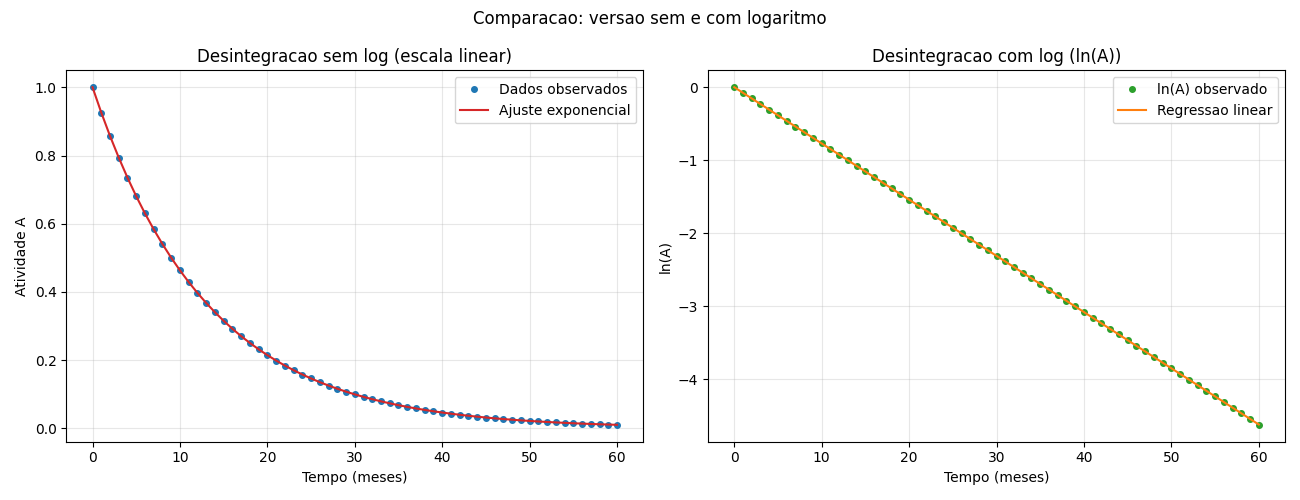
\includegraphics[width=0.9\linewidth]{Figura_1.png}
	\caption{Energia de liga\c{c}\~ao por n\'ucleon em fun\c{c}\~ao do n\'umero de massa.}
    \label{fig:placeholder}
\end{figure}


\section{Conclusão}

Este método de linearização permite uma estimativa robusta dos parâmetros nucleares da amostra estudada, minimizando erros de interpretação visual da curva exponencial original.

\end{document}